DM produced at colliders would register just as neutrinos do, which is to say: not at all. 
In this chapter, we describe DM production from a pragmatic, collider physicist's perspective, focusing on a selection of simple models with distinct and testable LHC signatures\footnote{For other perspectives, see the Reference Material.} 
Moreover, we will use the term {\it invisible particles} rather than DM when emphasizing that detecting such particles need not be a discovery of DM\footnote{For example, {\IP}s may decay after leaving the detector, a decay that is essential prompt on cosmological time scales.}.


The body of DM model literature can be divided into two extremes. %, each driving experimental searches in two complementary directions.
Fully-realized, self-consistent models such as SUSY provide specific features that can be exploited for narrowly-targeted searches, while simplified models with a few ingredients can capture broad collider signatures of classes of models, serving as benchmarks for more general but less optimal searches.
Key to both are the determinative details of the interactions between the DM and the SM, rather than the DM itself.


To restrict the scope of this review,
\begin{enumerate}
\item we describe only models where the DM interacts with SM hadrons, either directly or effectively;
\item we privilege models that include a $Z_2$ symmetry to stabilize DM;
\item we emphasize models connecting to a thermal, frozen-out relic; others, based on alternate cosmological histories (e.g. freeze-in), also have interesting LHC signatures~\cite{Bernal:2017kxu}
\item we stress models employed for early LHC Run-2 searches, where the DM is a Dirac fermion, and the model mimics the pattern of flavor violation found in the SM (Minimal Flavor Violation, or MFV~\cite{DAmbrosio:2002vsn}).
\end{enumerate}
Departures from these assumptions are discussed further in~\cite{Abercrombie:2015wmb}. 

\subsection{Higgs and Z boson portals}
\label{sec:HZPortalModels}

Extending the SM with a single DM particle, and nothing else, one may arrive at portal models where the Z or Higgs boson mediates the DM--SM interaction.
This is our first example of a {\it mediator}, a 'dark sector' particle that governs the DM-SM interaction.
While the \textbf{Z portal} is perhaps the simplest model of DM that one can construct, LEP and direct detection experiments strongly constrain it, as discussed in Sec.~\ref{sec:results_ZHSearches} and in~\cite{Escudero:2016gzx}.
\textbf{Higgs portal} models~\cite{Patt:2006fw,Djouadi:2011aa} are more promising, as only the recent generations of collider and direct detection experiments has reached the energies and luminosities necessary to search for them.
Direct collider searches for the invisibly-decaying Higgs bosons are augmented by measurements of other Higgs properties, which can be very sensitive to couplings to new particles.

The Z and Higgs portal models have relatively simple phenomenology.
The mediators (the Z or Higgs boson) are light in comparison to the LHC energy and can be produced on-shell.
Even if the {\IP}s are much heavier, and invisible decays of the mediator are absent, collider searches may still study the Z and Higgs and constrain these models through their fully-visible decays.

\subsection{Effective Field Theories and Simplified models of BSM mediators}
\label{sec:BSMMediatorModels}

One step further in complexity beyond the Z and Higgs portal models are models where the mediator is also a new particle, such as a heavier version of the $Z$ boson (a $Z^\prime$) or an additional scalar.

\begin{figure}[!htpb]
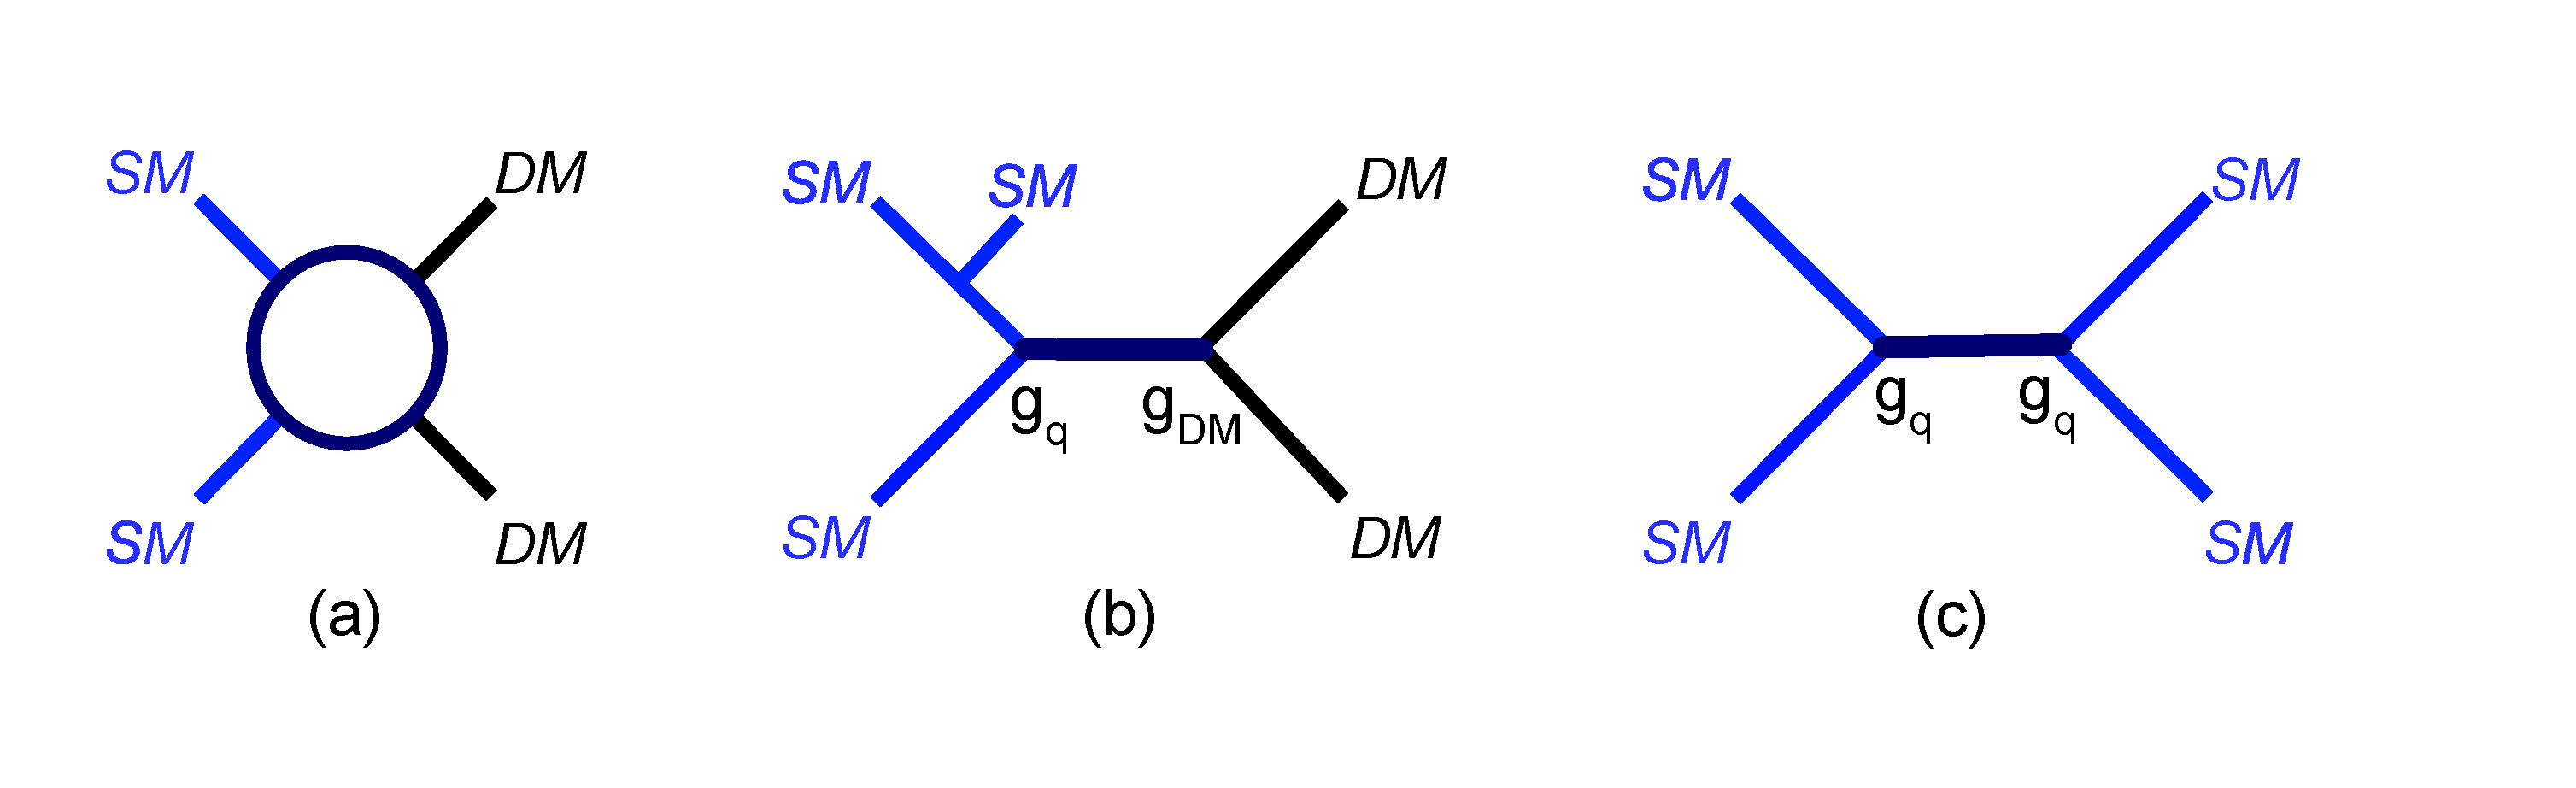
\includegraphics[width=\textwidth]{figures/MonoX.pdf}
\caption{Sketches of (a) the DM--SM interaction in an effective field theory (EFT), (b) a corresponding simplified model mediated by a BSM particle (with additional radiation off one initial state quark) and (c) the same model where the mediator decays back into SM, with coupling constant for the mediator-quark-quark vertex, \gq, and constant for the mediator-DM vertex, \gdm.}%From~\cite{monoXfig}.}
\label{fig:monoX}
\end{figure}

\subsubsection{Effective Field Theories}
\label{sub:EFT}

In some situations, such as when a BSM mediator is heavy compared to the collision energy, the DM--SM interaction appears to be a contact interaction, with all observables completely determined by one rate parameter, the contact interacion scale, that controls the production rate, and a Lorentz structure choice, which has a modest effect on the transverse momentum distributions of the {\IP}s.
In this case, Effective Field Theories (EFTs)~\cite{Goodman:2010ku,Bai:2010hh,Fox:2011pm} provide a description of the production of {\IP}s.
A sketch of an EFT process is shown in panel (a) of Fig.~\ref{fig:monoX}.
One may hope that such as description is sufficient for the LHC; the unknown high-energy details of a complicated interaction are conveniently integrated out.
Moreover, since EFTs do not fix a mediation mechanism, they provide a framework to systematically explore a wide range of possible physics.

If, instead, the interaction physics is kinematically accessible (e.g., the mediator mass is within reach of the typical momentum transfer in the collision), one should replace the EFT description with a model specifying further details of the SM--DM interactions~\cite{Shoemaker:2011vi}.
Without those details, however, one can still use the EFT language to provide results for later reinterpretation once a completion is known~\cite{Racco:2015dxa,Busoni:2013lha}. 

\subsubsection{Simplified models}
\label{sub:simplifiedModels}

When the collision energy is near or higher than the mediator mass, complementary avenues to study the mediating interaction develop, analogous to the transition from the Fermi model of weak interactions at low energies to the Standard Model at higher energies.
For example, at the LHC, a heavy neutral \Zprime mediator would often decay into the partons that produced it, and fully-reconstructing these visible decays can provide more information about the interaction than the invisible decays alone. 

Under the reductionist assumption that only a few new particles will be important in the early phase of a discovery, simplified models can be developed for tree-level pair production of {\IP}s (e.g.~\cite{Alwall:2008ag, Alves:2011wf}). 
The set of such models currently employed for ATLAS and CMS searches is described in Ref.~\cite{Abercrombie:2015wmb}, which builds upon much work from the wider dark matter community (e.g.~\cite{Fox:2011pm,Abdallah:2015ter}) 
Though these simplified models must be embedded in a larger theory to satisfy theory constraints~\cite{Kahlhoefer:2015bea}, they are sufficient to describe the leading order collider phenomenology in many cases.

\begin{marginnote}[]
\entry{The ATLAS/CMS Dark Matter Forum}{provided reference implementations of the models in Ref.~\cite{Abercrombie:2015wmb} at \url{https://gitlab.cern.ch/lhc-dmwg-material/model-repository}} and are implemented in models for various event generators (e.g. DMSimp~\cite{NewMadgraphModels}). 
\end{marginnote}. 

The standard models include models with neutral mediator particles singly-produced at the LHC and decaying to pairs of {\IP}s, and to pairs of SM particles (Figure~\ref{fig:monoX} (b) and (c)). Two-body mediator decays are simple, attractive benchmarks. Colored mediators allow vertices involving only one DM particle and phenomenology akin to that of SUSY models with a squark mediator~\cite{Papucci:2014iwa,An:2013xka,Bell:2012rg}. 

Models of BSM mediation can be classified according to the spin of the mediator: spin-1 vector or axial vector mediators (\Zprime), scalar mediators (termed $\phi$ in the following) and spin-2 mediators. Spin-2 mediator benchmarks have not yet been adopted by LHC searches; they produce diboson signatures not present in other models~\cite{Han:2015cty}. %removed cite Kraml:2017atm,

For additional decay signatures, for 'dark sectors' of many additional particles, and for far larger LHC datasets than at present, many more simplified models become interesting. 

\textbf{Massive color-neutral spin-1 bosons with vector or axial-vector couplings} are nearly ubiquitous in BSM theories, so \Zprime as the mediators connect with a wide class of models~\cite{Shoemaker:2011vi}.
Since the \Zprime coupling to quarks must be non-zero for its production at the LHC, both invisible and dijet signatures are discovery channels.
This coupling (or loop-level coupling) to SM partons is also required for nuclear recoils in underground DM searches.

The models in use at ATLAS and CMS contain either vector, axial-vector, or mixed couplings to quarks and a single species of {\IP}.
The couplings of the \Zprime (\gq to all quarks, \gl to leptons, and \gDM to {\IP}s), the mass of the {\IP} \mdm, and the \Zprime mass \mmed are free parameters.
Lepton decays, if not included explicitly at tree level, arise through the quark coupling at loop level (see Ref.~\cite{Albert:2017onk} and references therein). Decays of the spin-1 mediator into neutrinos are also required by gauge invariance, and add an invisible decay channel that can enhance signatures of missing transverse momentum, depending on the size of the couplings~\cite{Albert:2017onk}. 
The spin structure of the \Zprime couplings does not significantly change the LHC phenomenology, but has a much larger effect in signals in non-collider searches. 

\Zprime mediated models can include additional couplings of the \Zprime to acquire mass through a new baryonic Higgs $h_B$~\cite{Berlin:2014cfa} that collapses to the simpler model above in the limit of very heavy \Zprime mass. 
They can also be embedded in a Type-II Two-Higgs Doublet Model (2HDM)~\cite{Berlin:2014cfa}.%~\cite{Berlin:2014cfa,Liew:2016oon}.

With certain values of the model parameters, especially low \Zprime mass,
the model can satisfy the relic density constraints~\cite{Chala:2015ama}.
However, if taken in isolation, the model is non-renormalizable, and the axial-vector
model violates perturbative unitarity in certain regions of the off-shell parameter space~\cite{Chala:2015ama,Kahlhoefer:2015bea,Boveia:2016mrp}. 

\textbf{Color-neutral scalar and pseudoscalar bosons} are an BSM analogue of the Higgs portal model. In comparison to the \Zprime models, a BSM (pseudo-)scalar mediator model~\cite{Buckley:2014fba},  
has some additional peculiarities. 
Under MFV, the couplings of the (pseudo-)scalar bosons to fermions are mass-dependent. As with the Higgs boson, this has three familiar consequences: mediator production through loop-induced couplings to gluons~\cite{Haisch:2015ioa} and associated with heavy flavor quarks~\cite{Buckley:2014fba};
    production cross-sections are smaller than for vector mediators;
    and visible decays of the mediator are dominantly to third generation quarks. 
Despite lower production cross-sections, the more specific experimental signatures allow for these models to be tested during LHC Run-2.

The (pseudo-)scalar models used by ATLAS and CMS are fully specified by the masses of the \IP and the mediator, the $\phi$-\IP coupling (\gdm), and the $\phi$-fermion (\gq) coupling.
Following the convention in~\cite{Abercrombie:2015wmb}, \gq is a pre-factor to the Yukawa couplings to fermions and set equal for all quarks.
For the same model parameters, the scalar and pseudo-scalar models predict similar kinematic distributions.

When introducing an additional scalar, one must consider how the scalar relates to the Higgs boson. Large mixing with the Higgs can lead to strong constraints from Higgs measurements, for example when the scalar couples to DM through a Higgs portal~\cite{Berlin:2014cfa}.
If the mediators are pure SM singlets, the model is not invariant under $SU(2)_L$~\cite{Bell:2016ekl}. 
To restore gauge invariance, mixing with the Higgs sector is crucial. 
Couplings to the electroweak gauge bosons can also be added as a consequence of electroweak symmetry breaking~\cite{Bauer:2016gys,Englert:2016joy}. The tree-level signatures in this case include Higgs or vector bosons plus missing transverse momentum and, if the {\IP}s are sufficiently light, invisible decays of the Higgs boson.


\textbf{Colored scalar and pseudoscalar bosons} allow direct coupling between SM carrying color and {\IP}s carrying $Z_2$ charge~\cite{Bai:2013iqa, Papucci:2014iwa, An:2013xka, Bell:2012rg}. Colored mediators can have a broader set of multi-jet signatures and kinematic features than the neutral mediator models, including the radiation of vector bosons by the mediator~\cite{Bell:2012rg}. 

In colored (pseudo-)scalar models, the mediator must be heavier than the \IP to ensure \IP stability. 
For the current LHC results, the coupling, \gdmq, between {\IP}s and quarks, the \IP mass, and the mediator mass are free parameters. 

The exchange of a scalar colored under SU(3) is analogous to squarks in the MSSM where only squarks and neutralinos are light.
In the MSSM, the coupling between DM and the squark is constrained to be small\cite{Abercrombie:2015wmb}.
Without the requirements of a SUSY framework, this coupling need not be small. 
For example, if the DM is a standard thermal relic, the couplings required to obtain the correct dark matter density are generally higher than what used by SUSY models.
Models with three generations of mediators can satisfy flavor constraints and the SM gauge symmetry~\cite{Ko:2016zxg}. 

\subsubsection{Less simplified models}
\label{sec:LessSimplifiedModels}

Simplified models can guide the design of generic searches but do not cover the full complexity of possible collider signatures that arise in more complete models.
On the other hand, relying too heavily on a small sample of complete models risks focusing searches too narrowly on an unrepresentative set of signatures.

There are a large number of "less-simplified" models that attempt to find a middle ground between models that are too simplistic and those that are unnecessarily complex. Because the set of such models grows quickly with the number of ingredients, and there is not a broad consensus on which models should be a priority, very few of them have been explicitly considered by LHC searches. Here, we highlight a few such models with different signatures than the simplified models described above. 

\textbf{Co-annihilation} models add two specifies of dark sector particle, one close in mass to the other. Examples can be found in Refs.~\cite{Buschmann:2016hkc,Khoze:2017ixx}. The interaction between these two states drives the cosmological history~\cite{Ellis:1999mm}, as processes involving both types of particles can efficiently annihilate into SM particles. The LHC signatures include missing transverse energy and multiple hadronic jets accompanied by multiple resonant or non-resonant hadronic jets, but can be very diverse, encompassing signatures typically found in wildly different BSM models (e.g., searches for lepto-quarks). In some cases, these signatures are untested by any current LHC search~\cite{Buschmann:2016hkc}. 

Most simplified models in use at the LHC assume MFV to ensure that the models are compatible with a vast and unwieldy assortment of experimental constraints on flavor-violating processes. Nevertheless, viable \textbf{non-minimal flavor-violating models} can be constructed, but one must then understand the impact of the many constraints \cite{Blanke:2017tnb}. Mediators that couple to dark matter and a top quark are one category of flavor-violating model that remains least constrained by low-energy measurements~\cite{Boucheneb:2014wza}. These yield a distinct 'mono-top' LHC signature. 
%~\cite{DHondt:2015nat}

Other~\textbf{models with multiple mediators} with small couplings to SM particles have been developed to escape existing LHC constraints~\cite{Duerr:2016tmh}. 
The recent discovery of the Higgs boson places LHC at the forefront of the exploration of the SM scalar sector. Ultimately we don't yet know whether this scalar sector is limited to the SM Higgs boson. A single scalar mediator may not encode all important features of the more complicated phenomenology of more \textbf{complex scalar sectors}. Extended scalar sector models often involve signatures with \MET accompanied by the Higgs or other SM bosons.
One step beyond the simple scalar mediator model is to take mixing between this mediator and the SM Higgs boson, dictated by gauge invariance, into account~\cite{Bauer:2016gys,Berlin:2014cfa}. 
A much larger step beyond this is to consider an extended Higgs sector such as a Two-Higgs Doublet Model (2HDM) where one or more of the scalars acts as the SM-DM mediator~\cite{Bauer:2017ota,Goncalves:2016iyg,Bell:2016ekl}. 
In these models, the new  mediator mixes with the Higgs partners rather than with the SM Higgs, so that the model remains compatible with Higgs measurements. Some models developed for LHC searches focus on one Yukawa structure (Type-II). The particle content includes two CP-even bosons (one of which is the SM Higgs boson), two CP-odd bosons (of which one is the pseudoscalar DM mediator), two charged Higgs bosons, and the \IP. Masses and couplings of these models are chosen to respect vacuum stability~\cite{Goncalves:2016iyg}, electroweak and flavour constraints, and to reproduce the observed dark matter abundance.

\subsection{Supersymmetric models and other complete theories}
\label{sec:SUSYModels}

So far, we have considered rather general simplified models inspired by interactions found in the SM. These are obviously far from all the possibilities.
 Further sources of inspiration for searches are the large number of BSM theories that have been developed to solve theoretical problems of the SM, and the mechanisms through which these provide {\IP}s. 

Superymmetry (SUSY) is one class of such theories, postulating partner particles to all SM degrees of freedom to stabilize
the mass of a light Higgs boson.  
Reviews of supersymmetric DM models can be found in \cite{Feng:2010gw}. %,Ellis:2010kf already in bertone
Instead, we will broadly sketch models relevant to
recent experimental progress and stress where we expect future developments. 

Supersymmetric relic dark matter, the archetype for the WIMP idea, has a long
history \cite{1984NuPhB.238..453E}. Of these, the most viable and well-studied has been neutralino dark matter. 
The neutralino, a spin 1/2 partner particle to the SM gauge bosons, is often assumed to be the lightest supersymmetric particle (LSP). 
R-parity conservation makes the LSP stable~\cite{Farrar:1978xj} and prevents proton decay. 

In the Minimal Supersymmetric extension of the Standard Model (MSSM), there are four neutralinos, each a mixture of SM boson superpartners: a wino, a bino, and two higgsino fermion states.
The lightest neutralino may be called 'bino-like,' 'wino-like,' or 'higgsino-like'
in regions of MSSM parameter space where one of these components dominates the mixture.
The phenomenology of these  is different from most of the simplified models in the previous section, and it depends on mixture and on the particle spectrum. 
The LHC signatures feature missing transverse momentum from the neutralino and a high multiplicity of other objects
(leptons, jets) produced in cascade decays of heavier superpartners.  

The MSSM is a complete theory with more than 100 independent parameters, 
but realistic SUSY models might be far simpler.%reduced to far fewer independent degrees of freedom using experimental knowledge and theoretical assumptions (e.g. universality of certain particle masses or parameters). 
Such models are used as predictive benchmarks for DM searches. 
One of these is the phenomenological MSSM (pMSSM), which assumes no sources of CP violation beyond the SM nor Flavour-Changing Neutral Currents, and retains universal couplings and masses for first and second generation superpartners, reducing
the number of MSSM parameters to 19. 

Another DM candidate in gauge- or gravity-mediated supersymmetric models is the gravitino, 
a 3/2-spin particle superpartner of the graviton. 
Gravitino interactions are suppressed by the Planck scale (10$^{18}$ GeV) before SUSY breaking.
This has consequences both on their viability as a thermal relic and on their phenomenology. 
In gauge-mediated SUSY, the gravitino can be a DM candidate for a
non-standard cosmological history~\cite{Dimopoulos:1996vz}.
Similar to the neutralino case, the identity and masses of heavier states decaying to the gravitino LSP determine its phenomenology. 
However, the gravitino interactions are very weak, posing problems for direct and indirect detection searches. 

Because of the huge variety of potential experimental signatures, SUSY searches also often adopt a simplified model approach, 
decoupling the particles that determine the lowest energy collider phenomenology
(generally LSP and NLSP) from the rest of a heavier particle spectrum~\cite{Alves:2011wf}. 
As in the general simplified models described earlier, extending the MSSM quickly generates a plethora of non-minimal possibilities.

\subsection{Long-lived particle models}
\label{sec:LLPModels}

Another class of models found within and beyond SUSY are models feature suppressed cascade decays of a heavier particle (the NLSP in SUSY) to a lighter particle (the DM LSP in SUSY). The suppression can be so large that the particle travels a macroscopic length within the detector before it decays. Within SUSY, one way to achieve this suppression is for the NLSP to decay through a heavy intermediary. Split supersymmetry models are a subset of SUSY models where the gluino must decay through a heavy, off-shell squark~\cite{Masiero:2004ft}. The heavier the mass of the squark, the longer-lived the gluino. 
Alternatively, the NLSP decay can be heavily suppressed by some power of the mass difference with the LSP. This mass difference also affects DM co-annihilation rates and therefore the DM abundance~\cite{Ellis:1999mm}.
Finally, another way to achieve long-lived decays is with parameterically small couplings, as in the case of gauge-mediated supersymmetry models where the long-lived NLSP decays to its SM partner plus the gravitino~\cite{Dimopoulos:1996vz}, with a SM analogue in the Cabibbo-suppressed B-meson decays.
Because of the prevalence of these mechanisms, it is important to look for long-lived cascade decays.

Besides SUSY, one can find long-lived signatures within the generic simplified models in Sec. \ref{sub:simplifiedModels} for small enough couplings. If one assumes thermal freeze out, the coupling of the mediator to DM pairs is bounded from below to obtain a sufficiently large annihilation cross section. However, it's anybody's guess what mechanism in the early universe was responsible for the observed DM density. In alternate scenarios, such as "dark freeze out" where DM can annihilate directly to BSM mediators but not viceversa, the mediator couplings to the SM can be far smaller than allowed in standard thermal freeze out~\cite{Pospelov:2007mp,Das:2010ts}. The freeze-in scenario~\cite{Co:2015pka,Bernal:2017kxu} is another possibility for very weak DM--SM interactions.
Despite such small couplings, a sufficiently light mediator can be produced at colliders with appreciable cross section. Many models have been proposed in this direction. For example, DM can interact with the SM via a dark vector boson of a U(1)' dark symmetry, equivalent to the SM's U(1) but with much smaller couplings~\cite{Holdom:1985ag}, such as those originated by kinetic mixing. 
The mediator can also be a dark scalar boson (a "dark Higgs") that only couples to the SM, akin to a Higgs portal~\cite{Curtin:2014cca}. 
In both cases, the dark boson mediator can be light and long-lived~\cite{Pospelov:2007mp}, and its visible decays into SM particles or associated production with a SM boson provide the main collider handle for observation~\cite{Curtin:2014cca}. 
These scenarios can also be probed by complementary beam dump and fixed target experiments~\cite{Battaglieri:2017aum}. 
Simplified co-annihilation models with long-lived particles have also been proposed~\cite{ElHedri:2017nny}. 

\subsection{Dark interactions}
\label{sec:darkint}

In the above, we've sketched some of the models and signatures that are currently being sought at colliders. Next, we review experimental searches for {\IP}s, in light of the models discussed above. Nevertheless, we have left many models uncovered. From one point of view, any model containing stable particles interacting feebly with the SM is a theory of DM. Drawing the connections between this model and astrophysical DM is challenging, but this is the key difference between models of DM and other models of BSM physics. 

The dark sector can be arbitrarily complex, as long as the particles and interactions it contains satisfy cosmological observations~\cite{Strassler:2006im, Evans:2017kti}. The models listed above are simple examples of such dark sectors, where the mediator particles (e.g. dark bosons) provide the connection with the SM. Many other models are worthy of mention here, including asymmetric DM models, where dark sector particles and antiparticles are not produced in equal amount, in the same fashion as matter and antimatter for SM baryons~\cite{Zurek:2013wia}, and models of "neutral naturalness" realizing a mirror copy of the SM without any low-mass equivalent of the SUSY colored partners~\cite{Craig:2014aea}.
